\documentclass[conference]{IEEEtran}
\IEEEoverridecommandlockouts
% The preceding line is only needed to identify funding in the first footnote. If that is unneeded, please comment it out.
\usepackage{cite}
\usepackage{amsmath,amssymb,amsfonts}
\usepackage{algorithmic}
\usepackage{graphicx}
\usepackage{textcomp}
\usepackage{xcolor}
\usepackage{subcaption}
\usepackage[colorlinks=false]{hyperref}
\hypersetup{
    hidelinks
}
\definecolor{til}{HTML}{1E8449}
\definecolor{maxim}{HTML}{6C3483}
\definecolor{baptiste}{HTML}{21618C}

\def\BibTeX{{\rm B\kern-.05em{\sc i\kern-.025em b}\kern-.08em
    T\kern-.1667em\lower.7ex\hbox{E}\kern-.125emX}}
\begin{document}

\title{Statistical Machine Learning Final Project\\
    {\large solved with Random Forest and SVM}
}

\author{\IEEEauthorblockN{1\textsuperscript{st} Tilman Marquart}
\IEEEauthorblockA{\textit{Computer Science Bachelor} \\
\textit{SDU Exchange Student}\\
Nuremberg, Germany \\
timar20@student.sdu.dk \\
\color{til}{written text will appear in green}}
\and
\IEEEauthorblockN{2\textsuperscript{nd} Given Name Surname}
\IEEEauthorblockA{\textit{dept. name of organization (of Aff.)} \\
\textit{name of organization (of Aff.)}\\
City, Country \\
\color{maxim}{written text will appear in purple}}
\and
\IEEEauthorblockN{3\textsuperscript{rd} Given Name Surname}
\IEEEauthorblockA{\textit{dept. name of organization (of Aff.)} \\
\textit{name of organization (of Aff.)}\\
City, Country \\
\color{baptiste}{written text will appear in blue}}
}

\maketitle

\begin{abstract}
final project abstract, use random forest and ...
maybe write some intro sentences about the problem we try to solve
\end{abstract}

\section{Introduction}
%Give a brief intuitive summary of the two chosen classification algorithms. Identify the critical parameters.
%Talk about random forest with PCA. => critical hyperparams: PCA, NTREE, MTRY, NODESIZE, SAMPSIZE
\textcolor{til}{
    Our overall goal was to choose one fast but not so precise algorithm and one slower but more precise algorithm. We interpret fast as low training and prediction time. To choose the right algorithm we took a look at the asymptotic time complexity of the statistical machine learning algorithms (Table \ref{table:timeComplexity}).}

\textcolor{til}{
    For the fast but not so precise algorithm we choosed Random Forest. In addition to classical Decision Trees, will Random Forest generalize better on unseen data (important for the distinct people problem) by controlling the amount of various trees ($n_{trees}$). At the same time $n_{trees}$ will have a direct influence on our training and prediction time as seen in Table \ref{table:timeComplexity}, so we have to find a good balance for this hyper parameter. Other critical hyper parameters for Random Forest are: The amount of input features ($p$); Amount of features tried ($m_{try}$); Nodesize (${nodesize}$) controlling the tree depth; And lastly the sample size (${sampsize}$). We will discuss them in detail in Section \ref{sec:hyper:rf}.}

\textcolor{maxim}{
    For the slower but more precise method we decided to use a Support Vector Machine (SVM). 
}

% \begin{itemize}
%     \item The amount of features ($p$) which we try to reduce with a PCA preprocessing.
%     \item Amount of features tried ($m_{try}$) for finding the best decision point for the new tree branch.
%     \item Nodesize controls the minimum amount of samples in the leaf nodes and therefore also controls the depth of the tree.
% \end{itemize}

%ntree over classical dec. tree because it seems to be more robust against overfitting on just train part because of the parallel generated random trees.

\begin{table}[htbp]
    \color{til}
    \caption{\color{til}Time complexity in Big-O-Notation}
    \begin{center}
    \begin{tabular}{|c|c|c|}
        \hline
        \textbf{Algorithm} & \textbf{Training} & \textbf{Prediction} \\
        \hline
        Decision Tree & $\mathcal{O}(n^2p)$ & $\mathcal{O}(p)$ \\
        \hline
        Random Forest & $\mathcal{O}(n^2pn_{trees})$ & $\mathcal{O}(pn_{trees})$ \\
        \hline
        Support Vector Machine & $\mathcal{O}(n^2p+n^3)$ & $\mathcal{O}(n_{sv}p)$ \\
        \hline
        k-Nearest Neighbors & - & $\mathcal{O}(np)$ \\
        \hline
        \multicolumn{3}{l}{$n$ size of training dataset, $p$ number of features used } \\
        % \multicolumn{4}{l}{$p$ number of features used } \\
        \multicolumn{3}{l}{$n_{trees}$ number of various trees, $n_{sv}$ number of support vectors } \\
        % \multicolumn{4}{l}{$n_{sv}$ number of support vectors }
    \end{tabular}
    \label{table:timeComplexity}
    \end{center}
\end{table}

\begin{figure}[htbp]
    \centerline{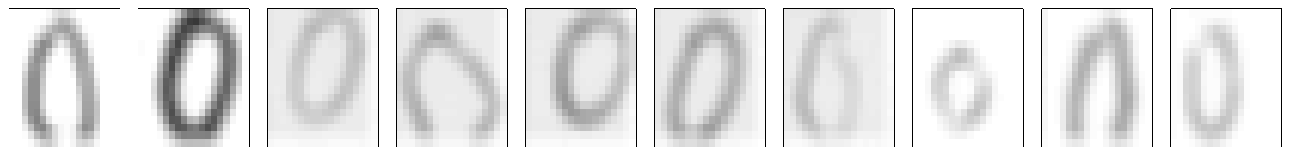
\includegraphics[width=1.0\linewidth]{preprocessing/mid_withoutNorm.pdf}}
    \centerline{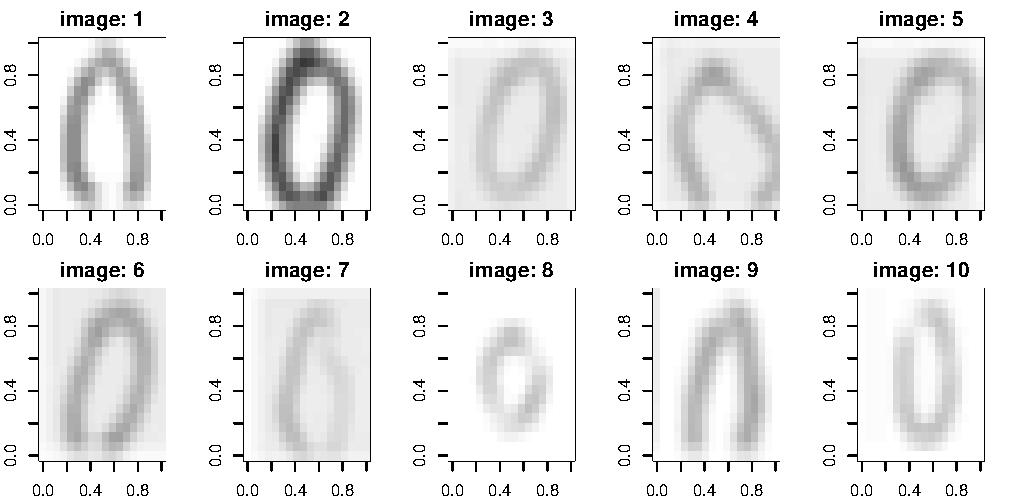
\includegraphics[width=1.0\linewidth]{preprocessing/corner_withoutNorm.pdf}}
    \centerline{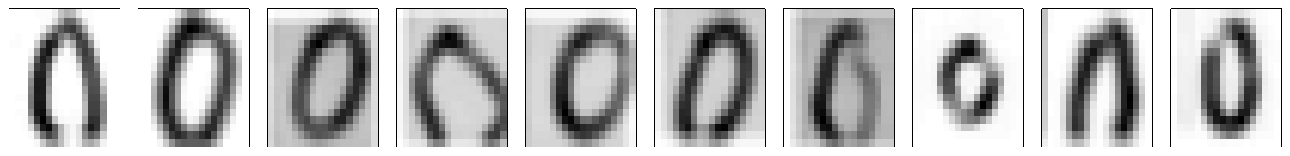
\includegraphics[width=1.0\linewidth]{preprocessing/corner_withNorm.pdf}}
    \caption{\color{til}Zero digits from first 10 students (left to right) in 100dpi mid dataset in first row; The same with the corner dataset in second row; Image wise min-max-normalization of corner dataset in third row}
    \label{fig:dataset}
\end{figure}

\begin{figure*}[ht!]
    \centering

    \subfloat[][]{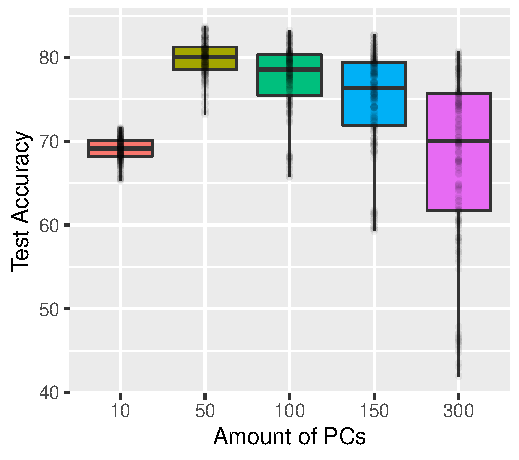
\includegraphics[width=0.3201\linewidth]{RandomForest/hypergrid/plots/final_run_28052020_pca_acc_barplot.pdf}}\quad
    \subfloat[][]{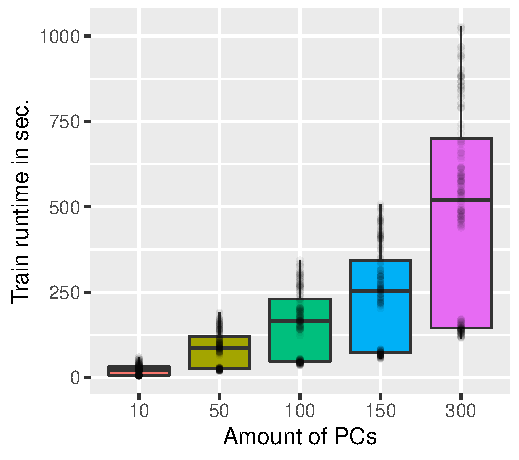
\includegraphics[width=0.3201\linewidth]{RandomForest/hypergrid/plots/final_run_28052020_pca_trainDuration_barplot.pdf}}\quad
    \subfloat[][]{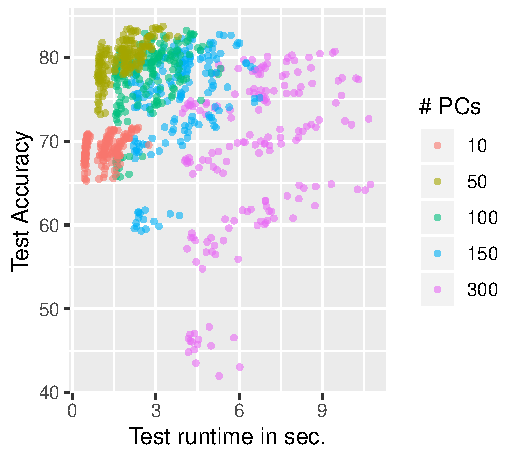
\includegraphics[width=0.3201\linewidth]{RandomForest/hypergrid/plots/final_run_28052020_pca_testDuration.pdf}}\quad

    \subfloat[][]{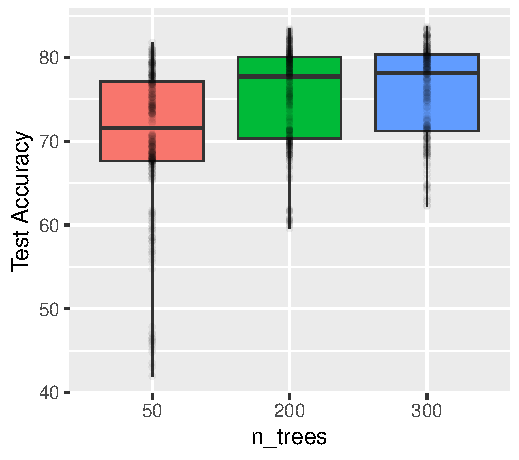
\includegraphics[width=0.3201\linewidth]{RandomForest/hypergrid/plots/final_run_28052020_ntree_acc_barplot.pdf}}\quad
    \subfloat[][]{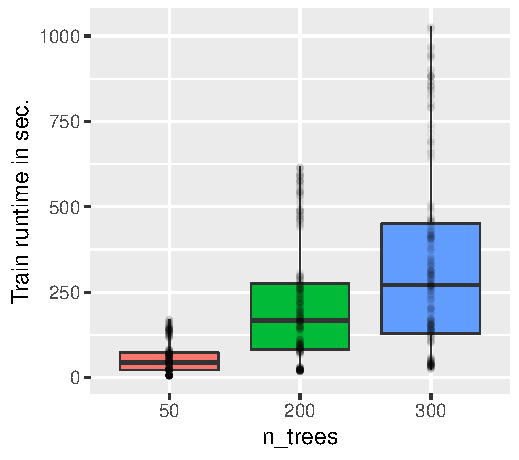
\includegraphics[width=0.3201\linewidth]{RandomForest/hypergrid/plots/final_run_28052020_ntree_trainDuration_barplot.pdf}}\quad
    \subfloat[][]{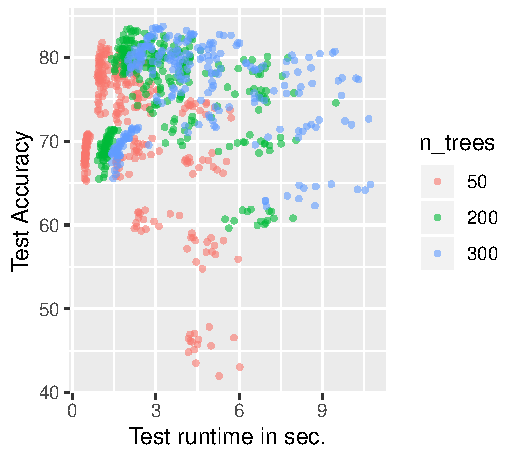
\includegraphics[width=0.3201\linewidth]{RandomForest/hypergrid/plots/final_run_28052020_ntree_testDuration.pdf}}\quad

    \caption{
        \color{til}
        Accuracy and runtime results of the 960 hyperparameter combinations; (a) Boxplot showing the accuracy for the hypergrid PCA sequence; (b) equivalent but for training runtime instead of accuracy; (c) accuracy over test runtime, ideal would be a point in the top left corner; (d,e,f) respectively to (a,b,c) but for amount of various trees $n_tree$ instead of $p$.
    }
    \label{fig:hyper:pca}
\end{figure*}

\section{Dataset and Preprocessing}
%TODO: Describe your preprocessing (dpi, PCA, centering, smoothing, normalization). Also show images. 
%TODO: why corner and not mid? => on a visual inspection corner seemed to be better centered and the digits better captured  => done
\textcolor{til}{
    During a visual inspection of the corner and mid dataset, the corner dataset seemed to better center the scanned digits and also cover the corners a bit better (See first two rows of Fig. \ref{fig:dataset}). We therefore decided to use the corner dataset for all out further analysis and the hyperparameter tuning. We later tried again the mid dataset on our tuned and optimized models and had worse results as with the corner dataset. This could proof our initial observations or more likely, the worse results are owed to the optimization of the model on the corner dataset. \\
    %TODO: why image wise min max norm? => some images with low saturation, digits probably written with a bright pencil
    While visually inspecting the dataset, we also discovered some images with low saturation, most likely these digits were written with a bright or colored pencil. In order to reduce the difference between images with high and low saturation, we apply a min-max-normalization on each image. Important to say is, that we are not using a traditional min-max-normalization with the minimum and maximum taken from the whole dataset but instead take the minimum and maximum from all 324 pixels of a single image and normalize the other pixel values with these minimum and maximum values. The result of this normalization is a dataset with equally saturated images as we can see in the third row of Fig. \ref{fig:dataset}. Especially for the disjunct problem this normalization improved the accuracy by 1,88\% for Random Forest.
}
\subsubsection{Random Forest Dataset and Preprocessing}
%TODO: why 100 dpi? => one goal was to be fast, small image size will increase fastness => done
\textcolor{til}{
    As seen in Table \ref{table:timeComplexity} the amount of features will have a direct influence on the runtime. Since we want to keep the runtime low for our Random Forest we try to reduce the amount of features with PCA beforehand. In behalf to minimize the runtime we used the dataset with 100dpi, since calculating the Principal Components will take way longer as higher the resolution of the input dataset is.
}

\subsection{Hyper parameter Optimization}
Optimize critical parameters (discussed under 1) on a smaller set and document this optimization process.

\begin{table}[htbp]
    \color{til}
    \caption{\color{til}Sequences for the hyperparameter grid}
    \begin{center}
    \begin{tabular}{|c|c|}
        \hline
        \textbf{Hyperparameter} & \textbf{Sequence} \\
        \hline
        Amount of Principal Components $p$ & 10, 50, 100, 150, 300\\
        \hline
        Random Forest $n_{trees}$ & 50, 200, 300\\
        \hline
        Random Forest $m_{try}$ & 1, 2, 4, 8\\
        \hline
        Random Forest ${nodesize}$ & 5, 20, 40, 60, 80\\
        \hline
        Random Forest ${sampsize}$ & 42000, 48000, 54000\\
        \hline
    \end{tabular}
    \label{table:hyperParamGrid}
    \end{center}
\end{table}


\begin{figure*}[ht!]
    \centering

    \subfloat[][]{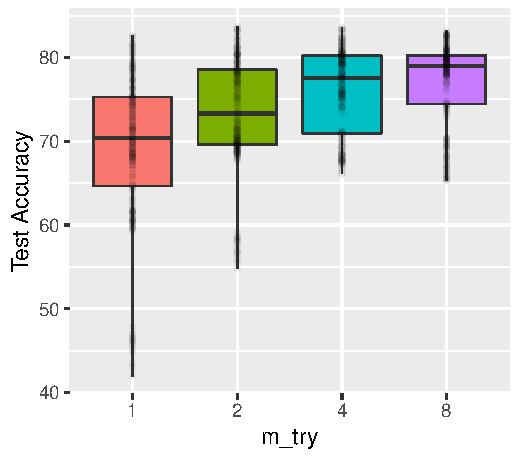
\includegraphics[width=0.3201\linewidth]{RandomForest/hypergrid/plots/final_run_28052020_mtry_acc_barplot.pdf}}\quad
    \subfloat[][]{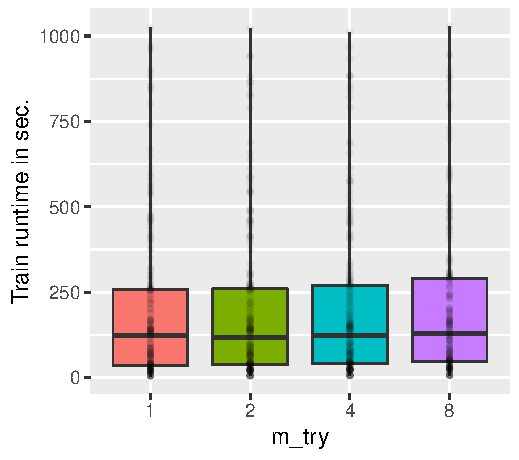
\includegraphics[width=0.3201\linewidth]{RandomForest/hypergrid/plots/final_run_28052020_mtry_trainDuration_barplot.pdf}}\quad
    \subfloat[][]{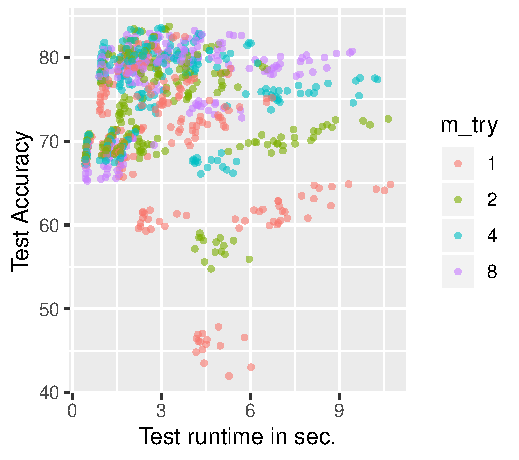
\includegraphics[width=0.3201\linewidth]{RandomForest/hypergrid/plots/final_run_28052020_mtry_testDuration.pdf}}\quad

    \subfloat[][]{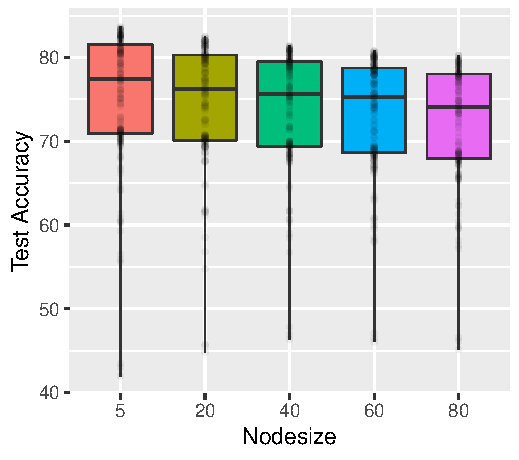
\includegraphics[width=0.3201\linewidth]{RandomForest/hypergrid/plots/final_run_28052020_nodesize_acc_barplot.pdf}}\quad
    \subfloat[][]{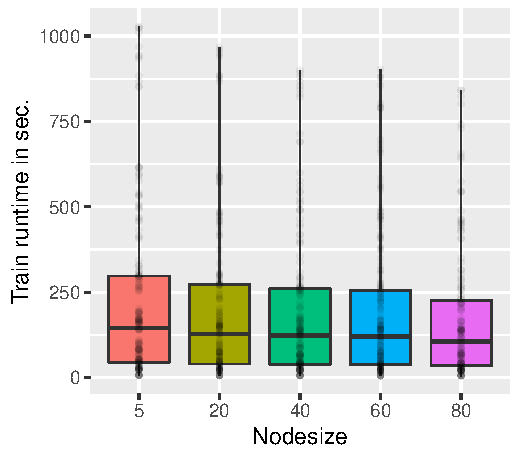
\includegraphics[width=0.3201\linewidth]{RandomForest/hypergrid/plots/final_run_28052020_nodesize_trainDuration_barplot.pdf}}\quad
    \subfloat[][]{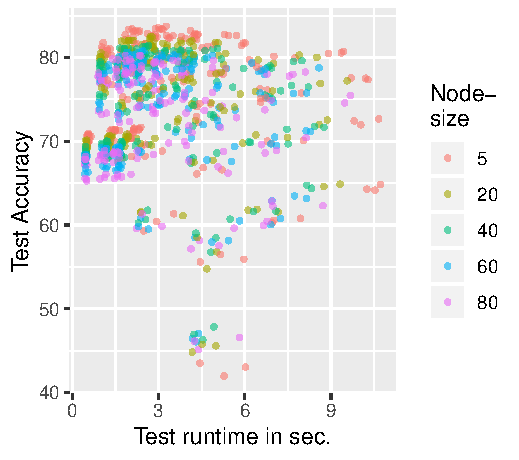
\includegraphics[width=0.3201\linewidth]{RandomForest/hypergrid/plots/final_run_28052020_nodesize_testDuration.pdf}}\quad

    \caption{
        \color{til}
        (a,b,c) respectively to Fig. \ref{fig:hyper:pca}(a,b,c) but for amount of features to try $m_{try}$ instead of $p$; (d,e,f) respectively to Fig. \ref{fig:hyper:pca}(a,b,c) but for ${nodesize}$ instead of $p$;
    }
    \label{fig:hyper:mtry}
\end{figure*}
\subsection{Hyper parameter Optimization for Random Forest}\label{sec:hyper:rf}
\textcolor{til}{
    Since optimizing random forest on the smaller dataset, was not bringing the right generalization, we decided to use a medium size dataset of 30 distinct people for training and the remaining 17 for testing and automate the finding of the right hyperparameters with a grid search. Therefore we create a hyperparameter grid with 960 combinations of the 5 hyperparameters (See Table \ref{table:hyperParamGrid} for details of the grid) and splitted them into 10 segments. We then used 4 Google Colab and 6 Kaggle notebooks in parallel, to let each segment of combinations run on each notebook. For each run we saved the Random Forest training and prediction runtime and the prediction accuracy on the test set. Google Colab and Kaggle are using nearly the same Intel Xeon CPU which was important to have a comparable runtime. In total the gridsearch took 47 hours and 53 minutes. The best test accuracy was 83.72\% (only pca preprocessing on a disjunct split of the 100 dpi corner dataset). In the following sections we will discuss the results of the gridsearch and how we used the results for a further manual fine tuning of the hyper parameters. 
    \subsubsection{Amount of Principal Components $p$}
    The amount of features $p$ will have a direct influence on the training and testing runtime as we can see in the computational complexity $\mathcal{O}(n^2pn_{trees})$ and $\mathcal{O}(pn_{trees})$. In order to keep Random Forest fast, we use Principal Components Analysis (PCA) to reduce the amount of features and use the first $p$ Principal Components (PCs) as our $p$ input features for Random Forest. The runtime results of our hypergrid search also proof the theoretical computational complexity as we can see in Figure \ref{fig:hyper:pca}b). The highest test accuracy of our results (Figure \ref{fig:hyper:pca}a) could be achieved by taking the first 50 PCs as input features. Adding more components even decreased the accuracy, which indicates an overfitting. With 50 PCs as Input Features, performs Random Forest still very fast (around 3 seconds) while also archiving it's best accuracy for our problem (See cluster of green dots in upper left corner of Figure \ref{fig:hyper:pca}c). Hence we took the 50 PCs and manually fine tuned our model further. Finally we came up with a final value of 40 PCs for our Random Forest PCA preprocessing.
}
\textcolor{til}{
\subsubsection{Random Forest $n_{trees}$}
As we would expect it from the computational complexity and as we can see it in our test results the amount of various trees $n_{trees}$, which the Random Forest algorithm growth, heavily effects train runtime (see Fig. \ref{fig:hyper:pca}e)) as well as test runtime (see Fig. \ref{fig:hyper:pca}f)). We therefore looking for the lowest value of $n_{trees}$ which still achieves a good accuracy. As we can see in Figure \ref{fig:hyper:pca}d) the accuracy does not vary a lot between 200 or 300 Trees, so we decided on a final $n_{trees}$ value of 200, because of the faster test and train runtime.
\subsubsection{Random Forest $m_{try}$}
In Random Forest training, the amount of features tried ($m_{try}$), controls how many features are checked for finding the best decision point for a new tree branch. Therefore it has no influence on the testing time. As we can see in Figure \ref{fig:hyper:mtry}, all values of $m_{try}$ (different colors) are evenly spread along the test runtime axis which confirms this assumption. Since we reached the highest mean test accuracy at the border of our $m_{try}$ grid domain, we manually tested even higher values for $m_{try}$ for our final model, but all of the higher values had even worse results, so we finally choose a $m_{try}$ value of 4 which yielded the best test accuracy.
\subsubsection{Random Forest ${nodesize}$}
The hyper parameter ${nodesize}$ controls the minimum amount of samples in the leaf nodes and therefore also controls the depth of the tree. By decreasing this value our tree will grow deeper and therefore the test and train time will increase. We can also see the increasing train (see Fig. \ref{fig:hyper:mtry}e) and test time (slight shift of red points to the right in Fig. \ref{fig:hyper:mtry}f) in our hyper grid search results. Even if it increases test and train time we choose 5 as our final ${nodesize}$, since it brought the best accuracy (see Fig. \ref{fig:hyper:mtry}d). During manual fine tuning we tried even smaller values but had worse results, probably because of overfitting.
\subsubsection{Random Forest ${sampsize}$}
During the grid search we tried out 3 different values for ${sampsize}$. This value will define how many samples from the input data are taken into consideration to generate the decission trees. Our grid search results did not showed a significant difference in accuracy between all of the 3 tested values. We therefore decided to use the default value of this hyperparameter.
}
%problem: on a smaller set!!! => maybe say smaller set was 30people and use crossvalidation with 43 to 4 with bigger set => argue why 30people was not a problem, because of colab and kaggle we choose 30people and let it run over night
%explain grid search for: PCA, NTREE, MTRY, NODESIZE, SAMPSIZE
%=> manual hyperparam optimization (by interpreting grid search barplots)
%=> preprocess optimization (by using image wise min-max norm)
%(remeber: Give information about the computational time required.)


\section{Evaluation}
Do a proper cross validation and indicate also mean and variances for all problems. Describe results on test and trainings set and reflect on overfitting. 
(remeber: Give information about the computational time required.)
(remeber: Analyze the results and give proper explanations)




\subsection{Random Forest}
=> use 10 fold crossvalidation with 43 to 4 with bigger set

(remeber: Give information about the computational time required.)
(remeber: Analyze the results and give proper explanations)

\section{Future Work}
Give an indication what could be further improved. 

optimize Random forst model also on corner dataset and see how it works


% \begin{thebibliography}{00}
% \end{thebibliography}

\end{document}
